\chapter{Prozess Anforderungen}
Wie wurde der Anforderungsprozess angepasst und durchgeführt? Vermutung gute Architektur hängt von nicht funktionalen Anforderungen ab treibender Faktor

\section{Modellierung der Usecases}
Usecase diagramm

\section{Überführen der Usecases in Anforderungstemplate}
Warum wurde ein Template und welches wurde verwendet

\section{Anpassen des Anforderungstemplates}
Welche Sachen konnten schon vorher ermittelt werden
\subsection{Wachstumsszenarien und Wahrscheinlichkeit}
\subsection{Änderungsszenarien}
\subsection{Businesskritikalität}
Ausfallkosten, Datenverlustszenarien
\subsection{Rahmenbedingungen}

\section{Modellierung der Daten}
Die zu speichernden Daten werden ermittelt und mit Hilfe eines Klassen Diagrammes modelliert. Dies ist nicht nur wichtig und nützlich, weil die Beispielanwendung in diesem Falle eine stark datenzentrierte Anwendung ist \cite[S. 105]{effektiv}, sondern wird später auch einen wesentlichen Beitrag zur Aufteilung des Systems in Komponenten leisten. Im Falle des Beispielprojekts wurden folgende Daten ermittelt und modelliert:

\begin{figure}[!htbp]
    \centering
    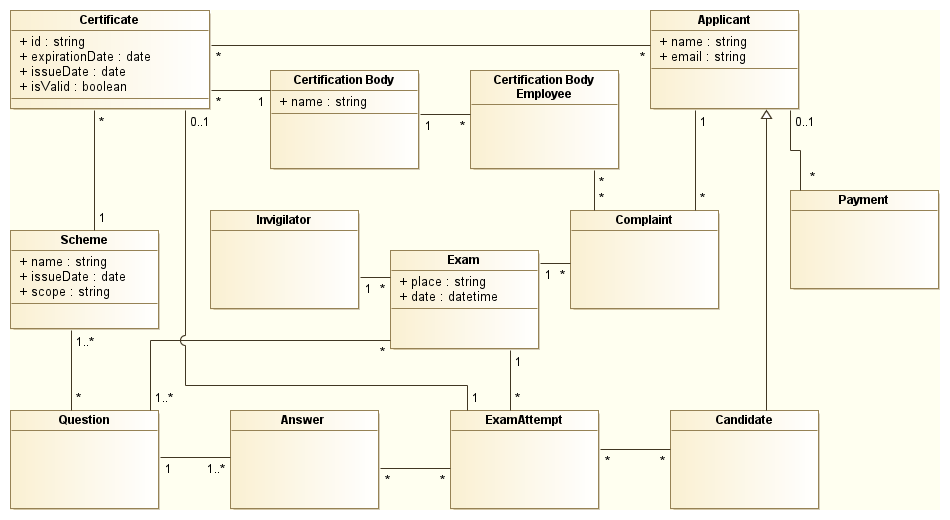
\includegraphics[scale=0.5]{uml/class.png}
    \caption{Das ermittelte Klassendiagramm des Beispielprojektes}
\end{figure}

\section{Datenaufteilung nach Lesendem Zugriff}
Nach der Ermittlung der Daten wird auf Basis der Rahmenbedingungen und Sicherheitsstruktur zusammen mit dem/der Kunden/Kundin ermittelt, welche Daten in welche Vertrautheitskategorien fallen. Dazu werden die Daten anhand ihrer gewollten Lesbarkeit in mehrere Untergruppen unterteilt.

Ermittelt wurden in diesem Falle folgende drei Kategorien:

\begin{itemize}
  \item Public: öffentlich zugängliche Daten, welche auf der Webseite zugänglich gemacht werden
  \item Internal: Daten, welche für die inneren Abläufe Betriebs notwendig sind, aber nicht öffentlich zugänglich sein sollen
  \item Confidential: Daten, welche innerhalb des Betriebes verwendet werden, aber eine besondere Geheimhaltungspflicht und Zugriffschbeschränkung benötigen. Dieses Vertrautheitslevel wurde aufgrund der Rahmenbedingung des Vertraulichen Umgangs mit Prüfungsdaten ermittelt \cite[7.3]{ISO_CERT}
\end{itemize}

Um diese Vertrautheitskategorien besser zu visualisieren zu können wird das UML Metamodel mit Hilfe eines Profiles angepasst. Jede Kategorie erhält einen gleich lautetenden Stereotypen \cite[S. 518]{glasklar}:

\begin{figure}[!htbp]
    \centering
    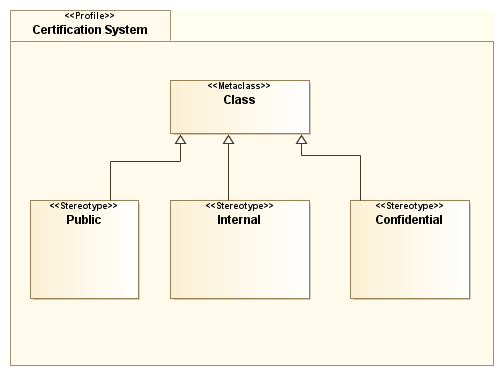
\includegraphics[scale=0.5]{uml/datastereotypes.png}
    \caption{UML wird mit einem Profil um drei Stereotypen erweitert}
\end{figure}

Nach der Erstellung der Stereotypen werden die Daten mit den Vertrautheitskategorien versehen. Sollte es nicht eindeutig sein, welche Klasse in welche Kategorie fällt, müssen die Daten aufgespalten werden und mit einer Assoziation modelliert werden.

\begin{figure}[!htbp]
    \centering
    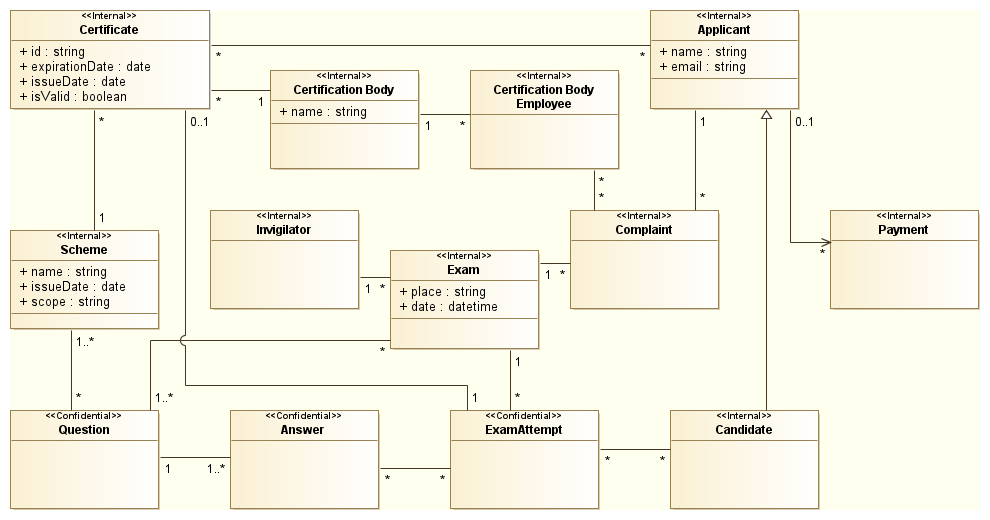
\includegraphics[scale=0.5]{uml/classstereotyped.png}
    \caption{Das Klassendiagramm wird mit Stereotypen der Vertraulichkeit erweitert}
\end{figure}

Überlegung:
* Daten werden in beiden Systemen benötigt:
 * Daten werden im System gespeichert, auf dem Schreibzugriff sein soll
 * System ohne Schreibzugriff synchronisiert diese Daten falls nötig, ansonsten einfach die services aufrufen
 * Auf beiden Systemen schreibzugriff -> bleibt im System

 TODO: vermerken dass das bsp projekt datenzentriert ist, nachschauen ob datenflussarch der richtige begriff ist

wer zugriff auf system mit daten hat kann daten abfangen
Schreibender zugriff?


\section{Modellierung der Akteure und Partnersysteme}
Kontextdiagramm der Akteure und Systeme
